\section{Near the trace: the fill, the filter, the cells and the integers}
\label{sec:nearfield}

On the synthetics, the reordered estimate's error near a rupture does not depend on the slip
(Section~\ref{sec:synthetic}). It is about 16\,mm of LOS inside the excluded fault zone and 7--9\,mm at 2--5\,km, the
same with no slip at all. Three parts of the estimator make it, and each can be changed: the fill's width, the filter's
weighted mean, and, where the deformation is steep, the cells themselves. Changed together, they bring that error
down to the far field's (Table~\ref{tab:nearfield}). Real data then say how much of it matters. On real ionosphere the
fills differ by about a millimetre, and next to the D141 rupture the screen is set by the main band's local integers
instead. The production screens of Sections~\ref{sec:nisar} and \ref{sec:sbtie} use none of the changes below.

\subsection{A fill matched to the gap}
\label{sec:fill}
Masked cells are filled by a local plane before the final Gaussian (Section~\ref{sec:estimator}). The production fill
uses one width, $\sigma = 10$\,km, chosen to reach across NISAR's partially focused near-range strip, where the screen
has to be extrapolated $\sim$11\,km from one side. Across a fault zone the data lie on both sides, and a narrower plane
should then follow a curved ionosphere better.

On synthetic ionospheres it does (Table~\ref{tab:fill}). The ionospheres are the default one, a rough one of 8\,rad at
8\,km and travelling waves of 3\,rad at 25\,km, with 0.7\,rad of noise per cell. In a 2\,km fault zone a 1.5\,km plane
misses by 2.0, 11 and 6\,mm rms, the 10\,km plane by 15, 60 and 29\,mm. The narrowest planes are best in every gap with
data around it, up to a 15\,km bay. Only deep in a one-sided strip do wider planes help, and there no plane does well:
30--130\,mm at 8--12\,km in. The plane's weighted data centroid tells the two cases apart: it stays near a cell inside
a gap with data on both sides, and moves away by about the distance to the data in a one-sided one. Each filled cell
therefore takes the narrowest of a ladder of planes whose data centroid lies within $1.5\sigma$ of it, blending into
the next width by $3\sigma$.

Real ionosphere is smoother at 2--10\,km than these synthetics, and its cells are noisier. We cut fake gaps out of
the raw estimates of the eight production screens of Section~\ref{sec:sbtie}: 34 windows of 100\,km, at least 15\,km
from a trace. Each window held a 40\,km fault zone of half-width 1, 2 or 4\,km at a random orientation, or had
everything beyond a line removed. We then refilled each gap and compared the result with the same filter run on all the
window's data (Table~\ref{tab:fill}, Fig.~\ref{fig:nearfield}b, c).
\begin{itemize}
  \item In 1--2\,km zones every fill errs by 1.1--3.1\,mm. A 2.6\,km plane, or a ladder that starts at it (2.6, 5 and
        10\,km), is best; the production plane is 0.6--1.1\,mm worse.
  \item The ladder that starts at 1.5\,km is too narrow for real data: 3.5--7\,mm in a 4\,km zone, against 2.1--3.6\,mm
        for the 2.6\,km ladder and 2.8--4.7\,mm for the production plane.
  \item At a one-sided edge, 6--10\,km planes are best (2.5--5\,mm at 0--8\,km), with the 2.6\,km ladder close behind
        (3.2--7.4\,mm). The narrowest plane and ISCE3's zero-order guide are 3--7 times worse there.
\end{itemize}
A matched fill is therefore worth about a millimetre in a real fault zone. Section~\ref{sec:integers} shows what it can
cost.

\subsection{A filter that does not lag where its weights change}
\label{sec:order}
ISCE3's final step is a Gaussian mean of the raw estimate, weighted by each cell's inverse Cram\'er--Rao variance. A
fault's damage zone lowers the coherence toward the trace, so the weights fall toward it. The mean's centroid then
moves away from the trace on both sides, and the screen lags the ionosphere's gradient in opposite directions on the two
sides. On the synthetic scene with D141-like near-field deformation, the raw estimate is unbiased to $\pm$2\,mm on each
side of the trace, while the filtered screen is 7--15\,mm high north of it and 8--11\,mm low south of it at 0.5--5\,km
(Fig.~\ref{fig:nearfield}a). With uniform weights, or with a weighted local plane through the same truncated kernel,
the asymmetry is gone.

The plane is a weighted Savitzky--Golay step: at each cell, the least-squares plane through the cells within the
kernel, weighted by the kernel times their inverse variances, evaluated at the cell. It is exact for a linear field,
whatever the weights, and equals the weighted mean wherever the weights are symmetric about the cell. Its variance
$e_0^\top M^{-1} N M^{-1} e_0$, with $M$ the weighted moments and $N$ the same moments under the squared kernel, takes
the place of the mean's in ISCE3's output sigma. \citet{piromthong2026ionospheric} fit such planes, with Gaussian
distance weights, against the same lag at scene edges. Next to a rupture it arises inside the data. With the matched
fill and the plane, the synthetic error within 2\,km of the trace falls to 2.0\,mm and at 2--5\,km to 1.5\,mm. The step
across the trace falls from 6.9 to 0.6\,mm, at 4\,m of slip as at none, against 1.3\,mm beyond 20\,km
(Table~\ref{tab:nearfield}).

How much the lag matters depends on the ionosphere's gradient where the weights change. Away from ruptures, on the real
fake gaps, the plane changes the error by at most 0.4\,mm. Next to the D141 rupture it moves the screen by at most
3\,mm, with the main band as cut or repaired (Section~\ref{sec:integers}).

\subsection{The main band out of every pixel}
\label{sec:pixel}
The cells sum each band's pixels before the scaled main band is taken out of the side band's cell phase. Where the
deformation changes by several radians across a 240\,m cell, the sums decorrelate. Their phases are then means of the
fringes that the two bands weight differently: the bands' speckle is independent, and the side band's pixels are eight
times wider in range. That difference enters $r$, and $d = r/k$ amplifies it 11.6 times. On a noise-free pair whose
fringes change by 2--20\,rad/km, the per-cell raw estimate errs by 0.25--2.5\,rad rms (5--48\,mm) per cell. North of
D141's trace the main band changes by a median 14--24\,rad/km within 2\,km. There only 2.5--18\% of the cells within
5\,km keep a coherence above 0.2 in both bands, against 19--64\% south of the trace.

Instead, \texttt{gslc\_cells} can take the caller's unwrapped main band $M$, interpolated to each pixel, out of every
pixel of both bands, scaled to each band's frequency, before the sums:
\begin{equation}
  \rho_A = \arg \sum_j a_j\, e^{i(\psi_{A,j} - M_j)}, \qquad
  \rho_B = \arg \sum_j b_j\, e^{i(\psi_{B,j} - (\fB/\fA) M_j)}, \qquad
  r = \W\!\left(\rho_B - \frac{\fB}{\fA}\,\rho_A\right),
  \label{eq:pixel}
\end{equation}
where $a_j$ and $b_j$ are the pixels' amplitudes. Pixel by pixel, $\psi_{B,j} - (\fB/\fA)\psi_{A,j} = k\,d_j$ exactly,
so the deformation leaves the sums before they are formed. What remains of the model's own error inside a cell enters
only as the difference of its two band-weighted means. On the noise-free pair, the raw estimate's error falls to
0.002\,rad, the precision of the model's interpolation. The model's integers are still the caller's, at 3.21\,rad per
cycle. Its sub-cycle errors no longer matter: with the true phase as the model, or with the main band's own pixels
after a one-pixel Gaussian, the synthetic screens agree to 0.05\,mm. The Gaussian multilook and the Goldstein filter
that precede the main band's unwrapping therefore reach the screen only through its integers. In both forms of the
cells, the values are the GSLCs' own pixels.

With the Okada field alone, which changes by $\sim$3\,rad/km at the trace, the two forms of the cells give the same
screen. With the D141-like near field, the per-pixel cells keep 34, 58, 96 and 100\% of the cells at 0--0.5, 0.5--1,
1--2 and 2--5\,km from the trace, against 6, 19, 45 and 83\% per cell. Their raw error at 2--5\,km is 17\,mm, against
29\,mm per cell and 15\,mm far from the trace. On D141 itself they double the cells kept north of the trace within
5\,km: 20 against 5\% at 0.5--1\,km, 35 against 18\% at 2--5\,km (Fig.~\ref{fig:nearfield}d). Those are the cells whose
main band is least certain.

\subsection{The main band's local integers}
\label{sec:integers}
On D141 the fill moves the screen near the trace by more than it moves the synthetics. A 2.6\,km plane and both
ladders raise it there by 7--16\,mm against the production screen, on both sides of the trace
(Fig.~\ref{fig:nearfield}e). The per-pixel cells add up to 4\,mm north of it, and the first-order filter moves it by
at most 3\,mm. The raw estimate shows why. Within 6\,km north of the trace it sits $\sim$15\,mm
above its own continuation from farther out, and it steps across the trace by 20--30\,mm. That step matches the 0.32
cycles left after the side band's whole-cycle tie (Section~\ref{sec:sbtie}).

The same pair was also unwrapped without the cut (v5 of Section~\ref{sec:sbtie}). Cell by cell, the two unwrappings'
integers differ beyond each block's modal difference north of the trace on 78\% of the cells within 1\,km, 62\% at
1--2\,km, 42\% at 2--4\,km and 18\% at 4--6\,km, and on 3\% or fewer beyond 6\,km. South of the trace they differ on
8--15\% beyond 1\,km and 33\% within it. Each such cell carries 3.21\,rad of raw estimate per cycle. When those cells
take the uncut unwrapping's integers, every recipe comes within 5\,mm of the production screen
(Fig.~\ref{fig:nearfield}f). The production screen itself moves by 2.4\,mm or less: its 10\,km fill averages the
near-trace cells away. The narrow fills and the extra cells follow them.

Neither unwrapping is known to be right near the trace. What the comparison shows is the order of things. Near a real
rupture the screen is set by the main band's local integers, at 3.21\,rad (62\,mm) per cycle and cell. The fill, the
filter and the cells refine it by a few millimetres once those integers are right. Until they are, the production
recipe's wide fill and fault-zone exclusion are the robust choice. The side band could check the integers patch by
patch near the trace, as it checks a cut-off block's in Section~\ref{sec:sbtie}. We leave that for later.

\begin{table}[t]
\centering
\caption{The near-trace recipe, one change at a time, on the through-going synthetic rupture at 4\,m of slip (mean
of five noise realizations): error rms in mm of LOS within 0--2, 2--5 and 5--10\,km of the trace, and the error's
2--4\,km step across it. Left: the Okada field alone. Right: with rough near-field deformation as large as D141's
(median 16--21\,rad/km within 1\,km of the trace). The error beyond 20\,km is 1.3\,mm with the first-order filter
and 2.1\,mm without it. The main band is the truth's.}
\label{tab:nearfield}
\setlength{\tabcolsep}{4pt}
\begin{tabular}{lrrrrrrrr}
\toprule
 & \multicolumn{4}{c}{Okada field only} & \multicolumn{4}{c}{with D141-like near field} \\
\cmidrule(lr){2-5}\cmidrule(lr){6-9}
recipe & 0--2 & 2--5 & 5--10\,km & step & 0--2 & 2--5 & 5--10\,km & step \\
\midrule
production (v6) & 15.6 & 7.5 & 1.8 & 6.9 & 19.0 & 10.5 & 4.3 & 11.9 \\
+ fill matched to the gap & 4.4 & 3.5 & 1.7 & 5.5 & 4.6 & 5.9 & 4.1 & 9.7 \\
+ first-order filter & 2.0 & 1.5 & 1.3 & 0.6 & 2.6 & 2.0 & 1.3 & 0.8 \\
+ main band out per pixel & 2.0 & 1.5 & 1.3 & 0.7 & 2.2 & 1.7 & 1.3 & 0.3 \\
+ no fault-zone exclusion & 1.5 & 1.2 & 1.3 & 0.5 & 1.6 & 1.3 & 1.3 & 0.2 \\
\bottomrule
\end{tabular}

\end{table}

\begin{table}[t]
\centering
\caption{The fills, rms error in mm of LOS. Synthetic ionospheres (eight of each, 0.7\,rad of noise per cell): inside
a 2\,km fault zone, and 4--8\,km into a one-sided 12\,km strip. Real ionosphere (34 windows of 100\,km in eight NISAR
screens, against the same filter on all the data): inside fake fault zones of half-width 1, 2 and 4\,km, and in a
one-sided strip.}
\label{tab:fill}
\small
\setlength{\tabcolsep}{3.5pt}
\begin{tabular}{lrrrrrrrrr}
\toprule
 & \multicolumn{4}{c}{synthetic ionospheres} & \multicolumn{5}{c}{real ionosphere, fake gaps} \\
\cmidrule(lr){2-5}\cmidrule(lr){6-10}
 & \multicolumn{3}{c}{2\,km zone} & edge & \multicolumn{3}{c}{zone half-width} & \multicolumn{2}{c}{edge} \\
\cmidrule(lr){2-4}\cmidrule(lr){5-5}\cmidrule(lr){6-8}\cmidrule(lr){9-10}
fill & default & rough & waves & 4--8\,km & 1\,km & 2\,km & 4\,km & 0--4\,km & 4--8\,km \\
\midrule
plane, 1.5 km & 2.0 & 10.8 & 6.1 & 37.2 & 1.1 & 1.8 & 5.4 & 18.6 & 34.0 \\
plane, 2.6 km & 2.9 & 17.0 & 9.2 & 20.9 & 1.1 & 1.8 & 2.8 & 6.0 & 33.1 \\
plane, 4 km & 4.5 & 25.8 & 13.9 & 12.2 & 1.3 & 1.9 & 2.9 & 3.9 & 9.6 \\
plane, 10 km (production) & 14.8 & 59.8 & 28.6 & 29.2 & 1.7 & 2.7 & 3.7 & 3.3 & 5.1 \\
ladder 1.5--3--6--12 km & 2.0 & 10.8 & 6.1 & 15.5 & 1.1 & 1.8 & 4.4 & 6.4 & 7.8 \\
ladder 2.6--5--10 km & 2.9 & 17.0 & 9.2 & 15.5 & 1.1 & 1.8 & 2.8 & 4.6 & 7.4 \\
ISCE3's guide & -- & -- & -- & -- & 1.3 & 2.0 & 5.1 & 10.5 & 23.3 \\
\bottomrule
\end{tabular}

\end{table}

\begin{figure}[t]
\centering
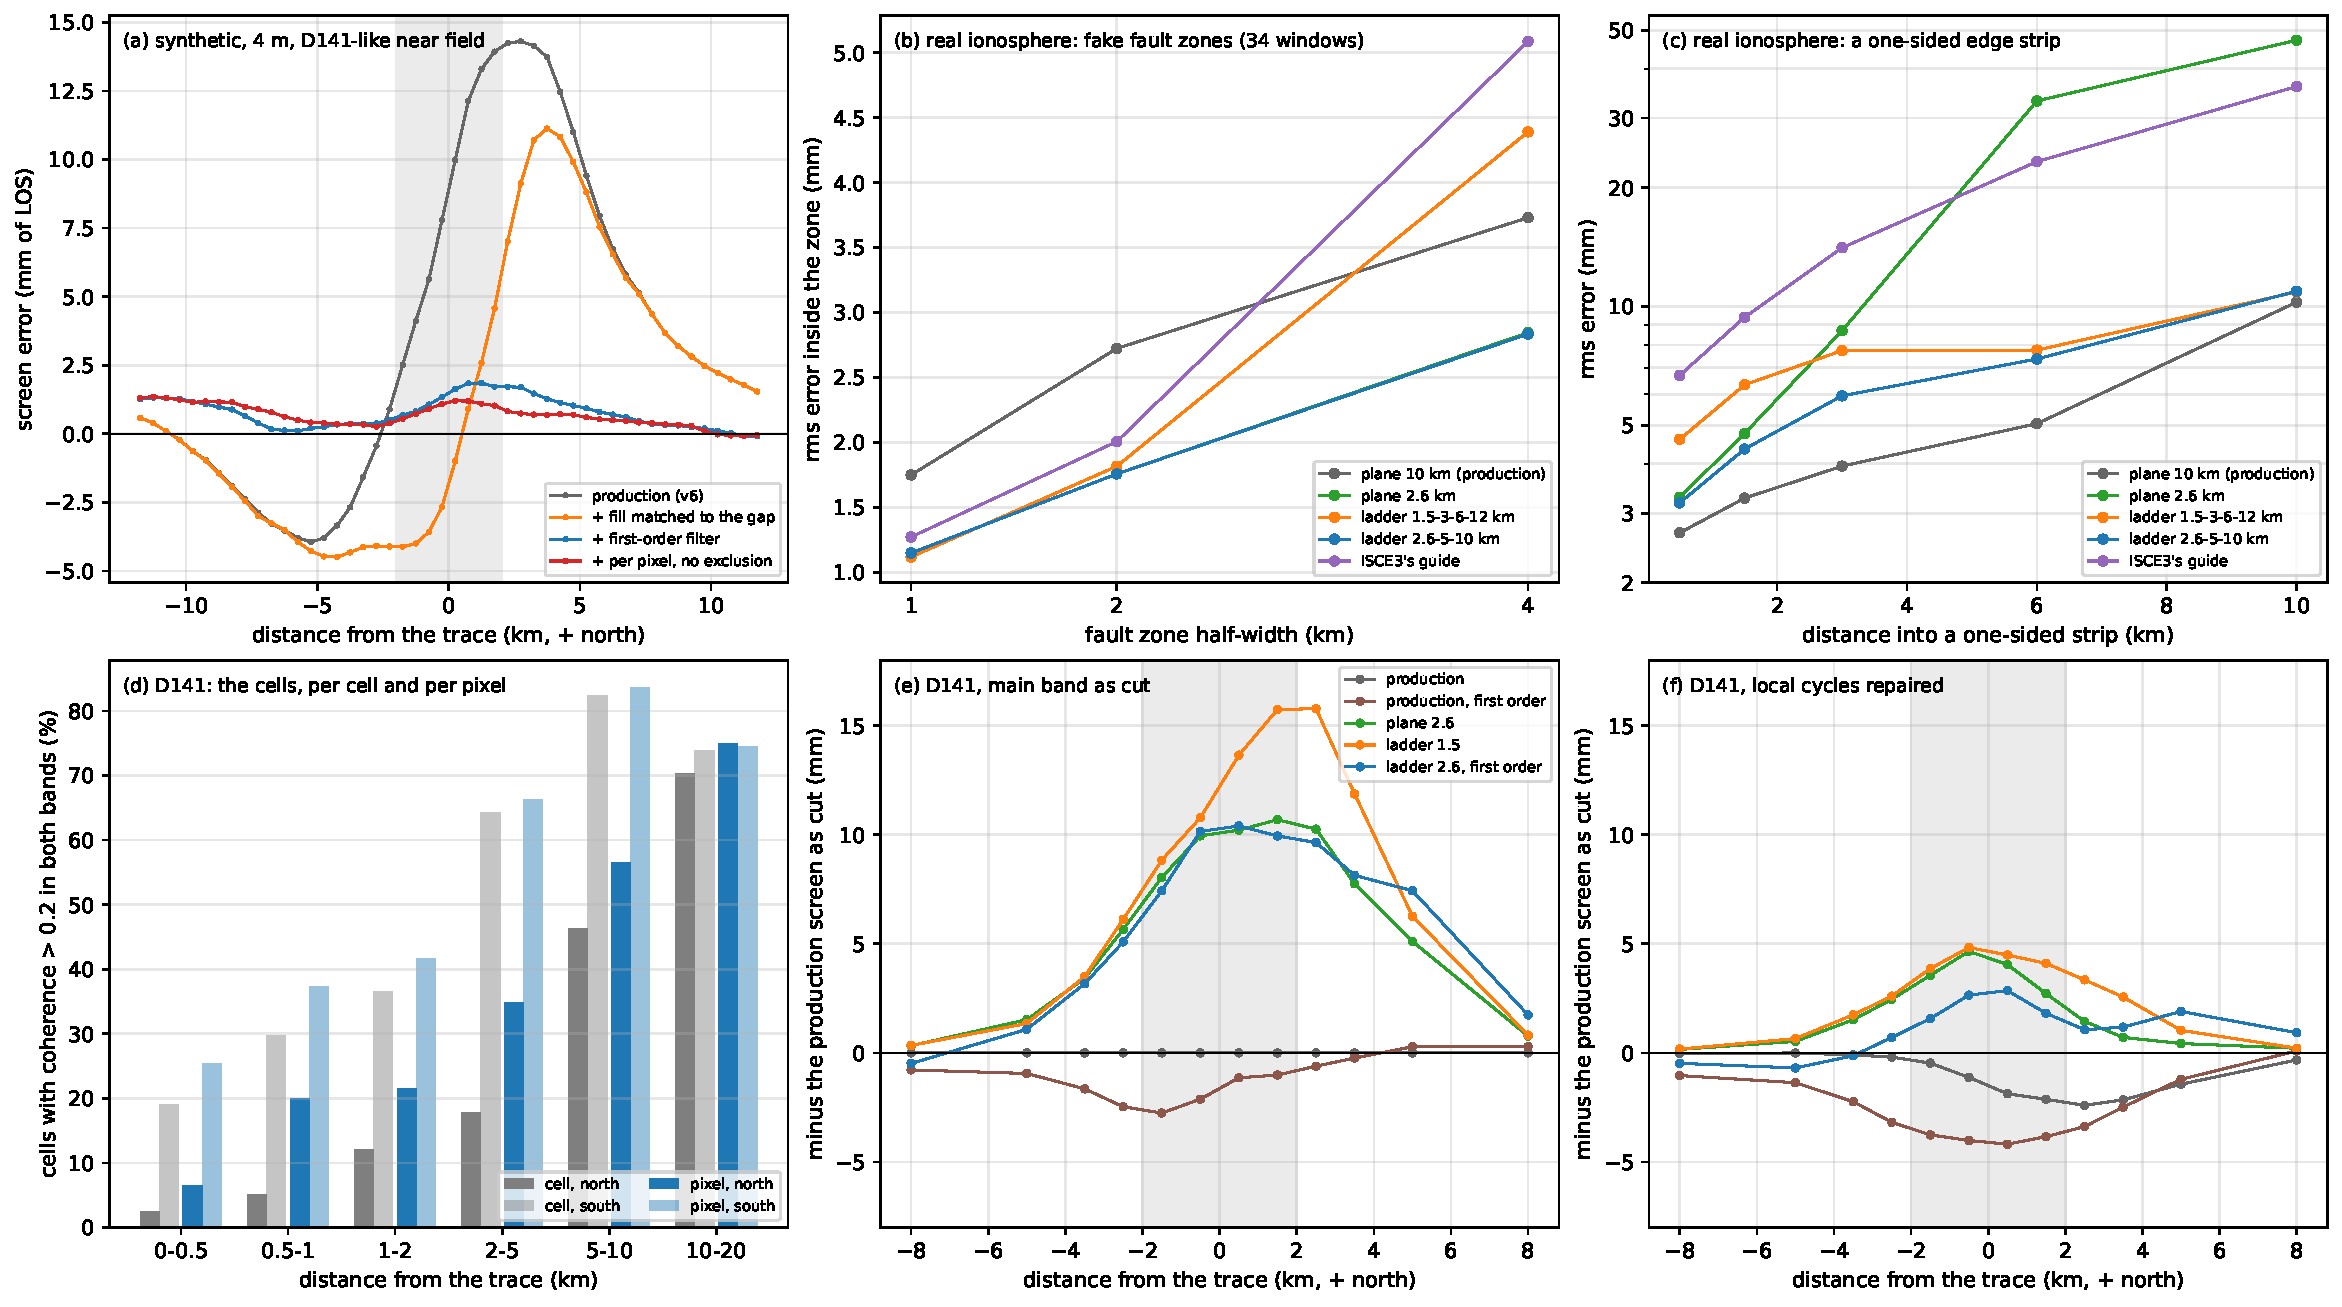
\includegraphics[width=\textwidth]{figures/fig_nearfield}
\caption{Near the trace. (a) The synthetic screen's error across the trace, D141-like near field, 4\,m of slip, one
change at a time; grey is the excluded zone. (b, c) The fills on real ionosphere: fake fault zones of 1--4\,km
half-width, and a one-sided strip. (d) D141: the cells with coherence above 0.2 in both bands, summed per cell and with
the main band taken out per pixel. (e, f) D141: each recipe's screen minus the production screen, with the main band
as cut and with its local cycles taken from the uncut unwrapping.}
\label{fig:nearfield}
\end{figure}
